\chapter{Architektura systemu (Frontend)}

\section{Stack Technologiczny}
\par
Warstwa wizualna aplikacji Labbyn została zrealizowana jako aplikacja typu SPA przy użyciu biblioteki React oraz języka TypeScript.
Głównym założeniem architektury było stworzenie wysoce interaktywnego u modularnego interfejsu użytkownika, zdolnego do płynnej obsługi złożonych struktur danych takich jak inwentarz, topologia laboratoriów czy mapa przestrzenna.
\par
Wybór biblioteki React był dla zespołu optymalny z dwóch głównych powodów: obszernego doświadczenia programistów w pracy z tym narzędziem oraz jego ugruntowanej, dominującej pozycji na rynku frameworków webowych (co potwierdzają m.in. globalne badania społeczności, np. ankieta Stack Overflow z 2025 roku).

\begin{figure}[H]
    \centering
    
\includegraphics[width=\textwidth]{images/WIP.png}
    \caption{Obraz 1.}
    \label{img:wip_1}
\end{figure}

\subsection{Wybór stosu: TanStack vs Next.js}
\par
Drugą poważnie rozważaną opcją technologiczną był framework Next.js.
W procesie projektowania zrezygnowano z popularnego frameworka Next.js na rzecz dedykowanego stosu opierającego się na ekosystemie TanStack.
Decyzja ta podyktowana była charakterystyką aplikacji Labbyn:
\begin{enumerate}
    \item Brak wymogu SEO: Labbyn to aplikacja wewnętrzna/narzędziowa , gdzie indeksowanie przez wyszukiwarki nie jest potrzebne.
    \item Stan aplikacji i interaktywność: Aplikacja mocno polega na złożonym stanie klienckim. Modele SSR i RSC oferowane przez Next.js wprowadzają narzut architektoniczny, który w przypadku "ciężkich" klientów bywa zbędny.
    \item Szybkość przejść: Pełne SPA obsługiwane przez TanStack Router pozwala na błyskawiczne przejścia między widokami bez konieczności odpytywania serwera o strukturę strony.
    \item Niezależność infrastrukturalna (Self-hosting): Next.js posiada wiele wbudowanych integracji z platformą Vercel, co jest użyteczne przy komercyjnych wdrożeniach. Jednakże, ze względu nanaturę open-source projektu Labbyn oraz zamysł samodzielnego hostowania aplikacji, większość z tych funkcji pozostałaby niewykorzystana. Co więcej, mogłoby to narzucić potencjalnym odbiorcom korzystanie z płatnych narzędzi ekosystemu Vercel (zjawisko tzw. vendor lock-in).
\end{enumerate}

\section{Architektura (trzeba rozpisać)}
\par
Architektura warstwy frontendowej została oparta na wzorcu programowania zorientowanego na komponenty, z wyraźnym podziałem odpowiedzialności między routing, pobieranie danych i warstwę prezentacji.
Takie podejście gwarantuje skalowalność kodu oraz ułatwia testowanie i rozbudowę systemu o nowe moduły.

\subsection{Mechanizm Autoryzacji Użytkownika}
\par
Proces uwierzytelniania i autoryzacji został zintegrowany bezpośrednio z systemem routingu.
\par
Główny układ aplikacji dla zalogowanych użytkowników zdefiniowano w pliku \url{src/routes/\_auth.tsx}.
Plik ten pełni rolę strażnika (ang. Route Guard).
Jeśli użytkownik nie posiada ważnej sesji, następuje przekierowanie do ścieżek publicznych: src/routes/login.tsx (obsługiwanej przez login-form.tsx) lub src/routes/setup-password.tsx. 
\par
W przypadku przekierowania na ekran logowania, w parametrach adresu URL przekazywana jest aktualna lokalizacja, do której próbował dostać się nieautoryzowany użytkownik.
Dzięki temu mechanizmowi, po pomyślnym zalogowaniu, użytkownik jest płynnie kierowany na docelową podstronę, co znacząco poprawia ergonomię pracy.

\begin{figure}[H]
    \centering
    
\includegraphics[width=\textwidth]{images/WIP.png}
    \caption{Obraz 2.}
    \label{img:wip_2}
\end{figure}

\par
Zagnieżdżenie struktury katalogów (wszystkie widoki panelu znajdują się w \url{src/routes/\_auth/}) daje architektoniczną gwarancję, że żadna podstrona z danymi wrażliwymi nie zostanie wyrenderowana przed poprawną weryfikacją tożsamości.

\begin{figure}[H]
    \centering
    
\includegraphics[width=\textwidth]{images/WIP.png}
    \caption{Obraz 3.}
    \label{img:wip_3}
\end{figure}

\subsection{Warstwa komunikacji frontend - backend}
\par
Aby zachować czystość kodu i separację obaw, komunikacja z warstwą backendową (REST API) opiera się na połączonym działaniu biblioteki Axios oraz TanStack Query, zlokalizowanych we wzorcu w katalogu src/integrations/.
\par
Axios odpowiada za niskopoziomową budowę żądań HTTP.
Wykorzystano mechanizm interceptorów do automatycznego wstrzykiwania nagłówków autoryzacyjnych oraz globalnej obsługi błędów.

\begin{figure}[H]
    \centering
    
\includegraphics[width=\textwidth]{images/WIP.png}
    \caption{Obraz 4.}
    \label{img:wip_4}
\end{figure}

\par
TanStack Query zarządza cyklem życia samych danych (odpowiedzi z API) i stanem asynchronicznym.
Odpowiada za budowanie treści żądań, pozwala na zaawansowane techniki buforowania/cacheowania przy użyciu unikalnych kluczy, a także dostarcza zintegrowane stany ładowania.

\begin{figure}[H]
    \centering
    
\includegraphics[width=\textwidth]{images/WIP.png}
    \caption{Obraz 5.}
    \label{img:wip_5}
\end{figure}

\begin{figure}[H]
    \centering
    
\includegraphics[width=\textwidth]{images/WIP.png}
    \caption{Obraz 6.}
    \label{img:wip_6}
\end{figure}

\par
Każda domena biznesowa (np. inventory, machines, user) posiada własny podkatalog zawierający:
\begin{itemize}
    \item \text{[domena].query.ts:} Definicje hooków do pobierania danych z wykorzystaniem useQuery.
    Zapewniają one mechanizmy cachowania, deduplikacji żądań oraz automatycznego odświeżania w tle.
    \begin{figure}[H]
        \centering
        
\includegraphics[width=\textwidth]{images/WIP.png}
        \caption{Obraz 7.}
        \label{img:wip_7}
    \end{figure}
    \item \text{[domena].mutation.ts:} Definicje hooków do modyfikacji danych (useMutation), obsługujące m.in. optymistyczne aktualizacje interfejsu.
    \begin{figure}[H]
        \centering
        
\includegraphics[width=\textwidth]{images/WIP.png}
        \caption{Obraz 8.}
        \label{img:wip_8}
    \end{figure}
    \item \text{[domena].types.ts:} Interfejsy TypeScript ściśle odzwierciedlające struktury danych z API.
    \begin{figure}[H]
        \centering
        
\includegraphics[width=\textwidth]{images/WIP.png}
        \caption{Obraz 9.}
        \label{img:wip_9}
    \end{figure}
\end{itemize}

\section{Struktura interfejsu i główne komponenty}
\par
Architektura warstwy wizualnej opiera się na podejściu modułowym, inspirowanym metodologią Atomic Design.
Podzielono ją na trzy główne kategorie:
\begin{figure}[H]
    \centering
    
\includegraphics[width=\textwidth]{images/WIP.png}
    \caption{Obraz 10.}
    \label{img:wip_10}
\end{figure}
\begin{enumerate}
    \item Komponenty bazowe (UI): Zlokalizowane w \url{src/components/ui/} (np. button.tsx, dialog.tsx, data-table.tsx). Stanowią one niezależne, generyczne klocki budulcowe,oparte o wzorzec biblioteki shadcn/ui. Zapewniają one spójność zachowań (np. dostępność a11y) w całej aplikacji. \url{https://ui.shadcn.com/docs/components}
    \item Komponenty układu (Layout): Obejmują m.in. app-sidebar.tsx (główna nawigacja), page-header.tsx oraz szablony takie jak subpage-template.tsx, które gwarantują ujednoliconą strukturę wizualną podstron. Na przyklad:
    \begin{figure}[H]
        \centering
        
\includegraphics[width=\textwidth]{images/WIP.png}
        \caption{Obraz 11.}
        \label{img:wip_11}
    \end{figure}
    \begin{figure}[H]
        \centering
        
\includegraphics[width=\textwidth]{images/WIP.png}
        \caption{Obraz 12.}
        \label{img:wip_12}
    \end{figure}
    \item Komponenty domenowe: Dedykowane konkretnym funkcjom, np. \text{add-inventory-dialog.tsx}, \text{manage-rental-dialog.tsx}, czy moduł importu/eksportu (\url{src/components/import-export/}).
\end{enumerate}

\section{Mapa przestrzenna}
\par WIP

\section{Tożsamość graficzna}
\par
Stylowanie aplikacji zostało oparte na zmiennych CSS.
Taka architektura pozwoliła na szybkie wdrażanie eksperymentów wizualnych oraz wbudowanie pełnej obsługi dwóch motywów wyświetlania: jasnego i ciemnego, które użytkownik może łatwo dostosować do własnych preferencji widzenia i warunków oświetleniowych w laboratorium.
Ze względu na charakter projektu gdzie użytkownikami końcowymi są w większości technicy używający aplikacji przez wiele godzin większy priorytet został nałożony na tryb ciemny.

\begin{figure}[H]
    \centering
    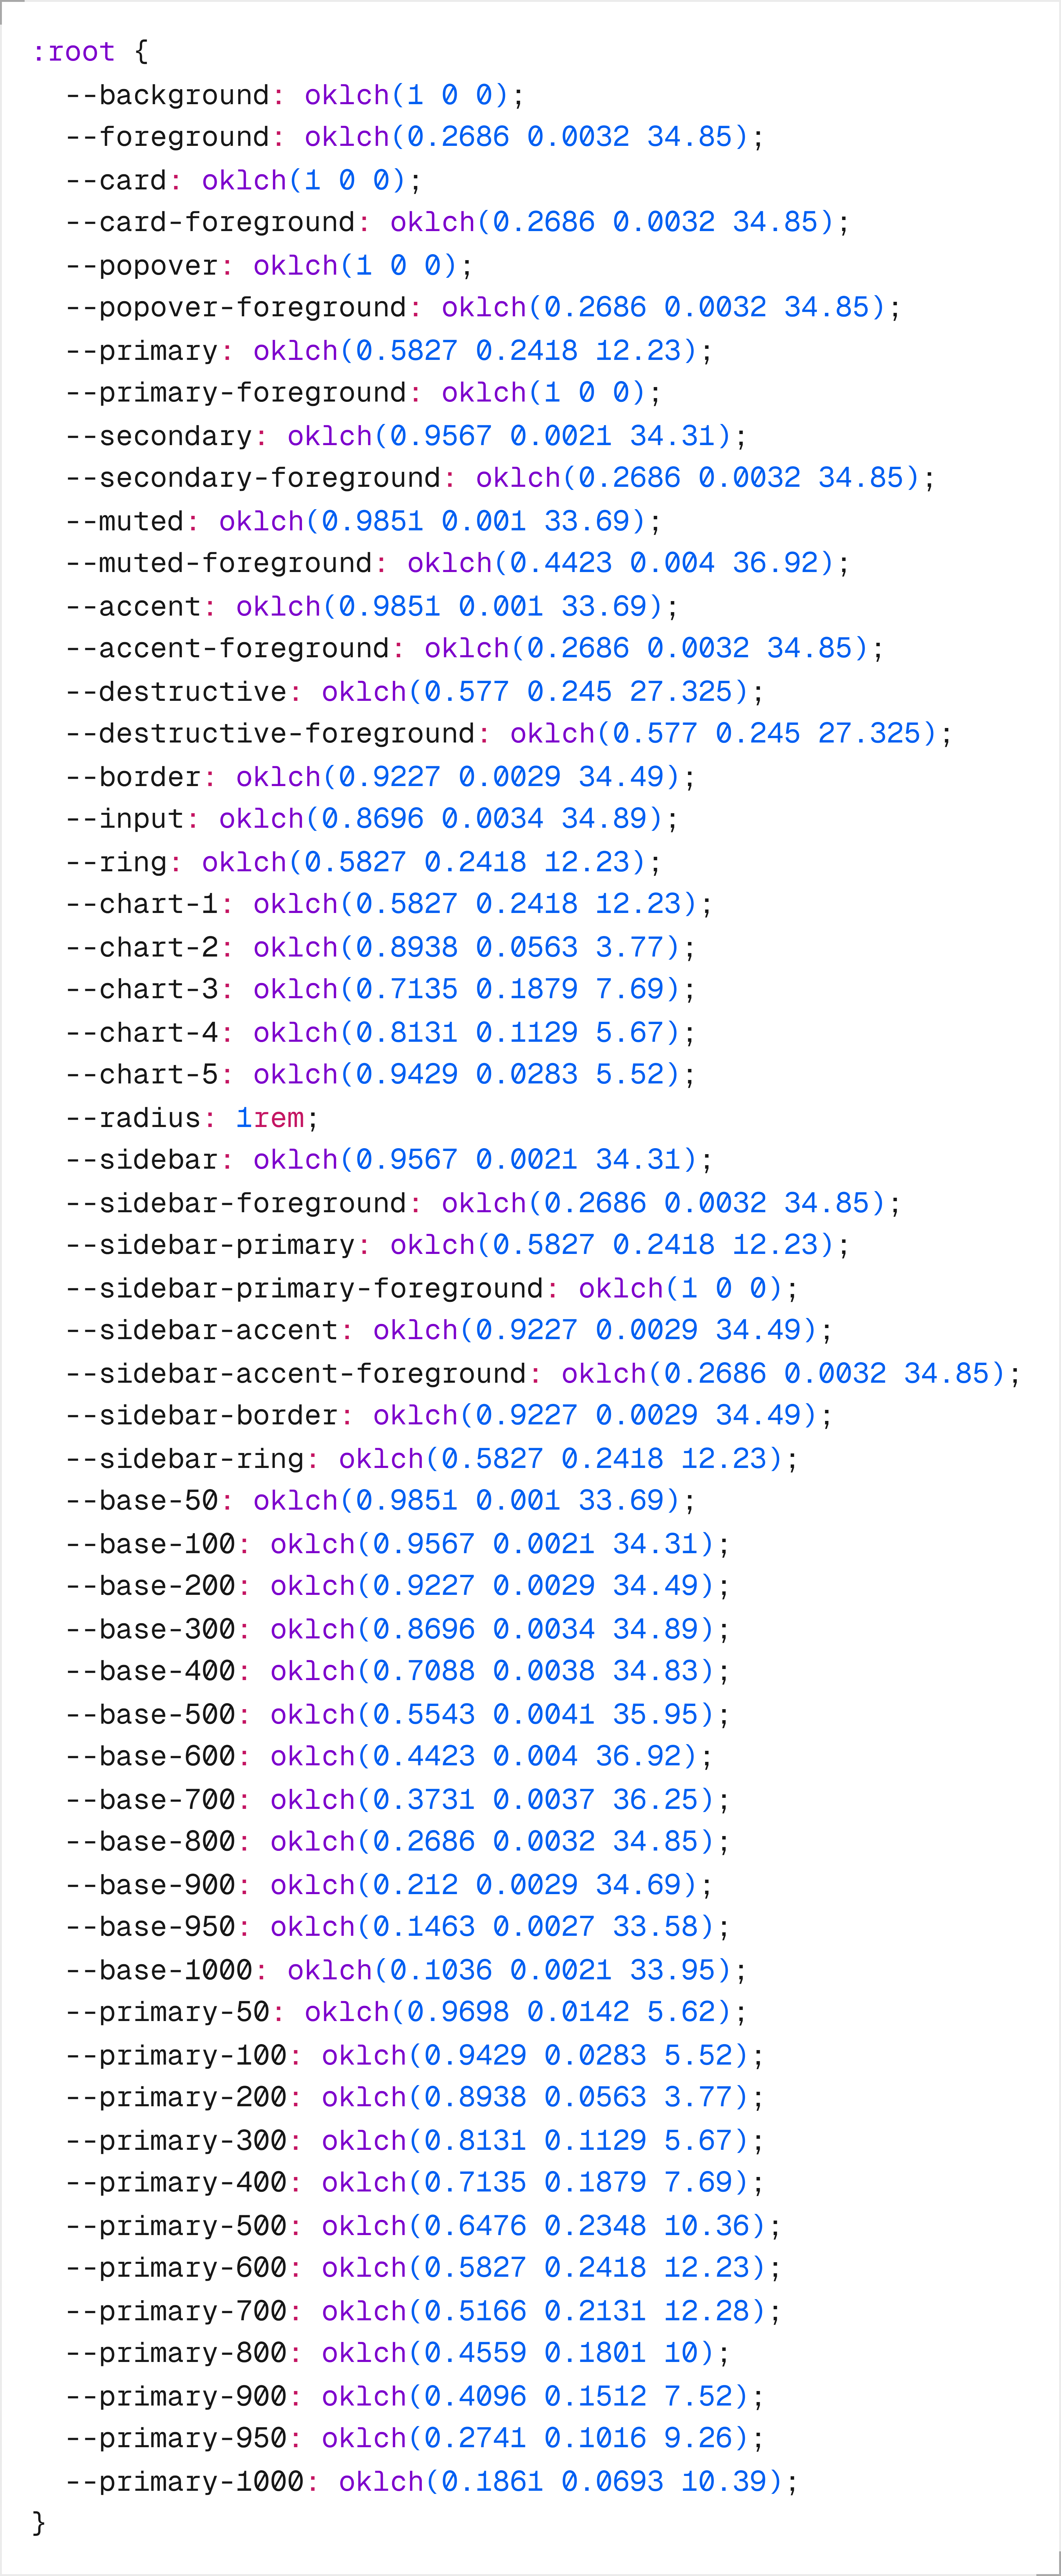
\includegraphics[height=0.9\textheight,keepaspectratio]{images/frontend/zmienne_css_kod.png}
    \caption{Zmienne pliku CSS aplikacji (opracowanie własne)}
    \label{img:zmienne_css}
\end{figure}

\par
Podczas opracowywania szaty graficznej został przygotowany prototyp logotypu projektu, natomiast nie został on dopracowany do finalnej wersji w ramach pracy inżynierskiej.
\begin{figure}[H]
    \centering
    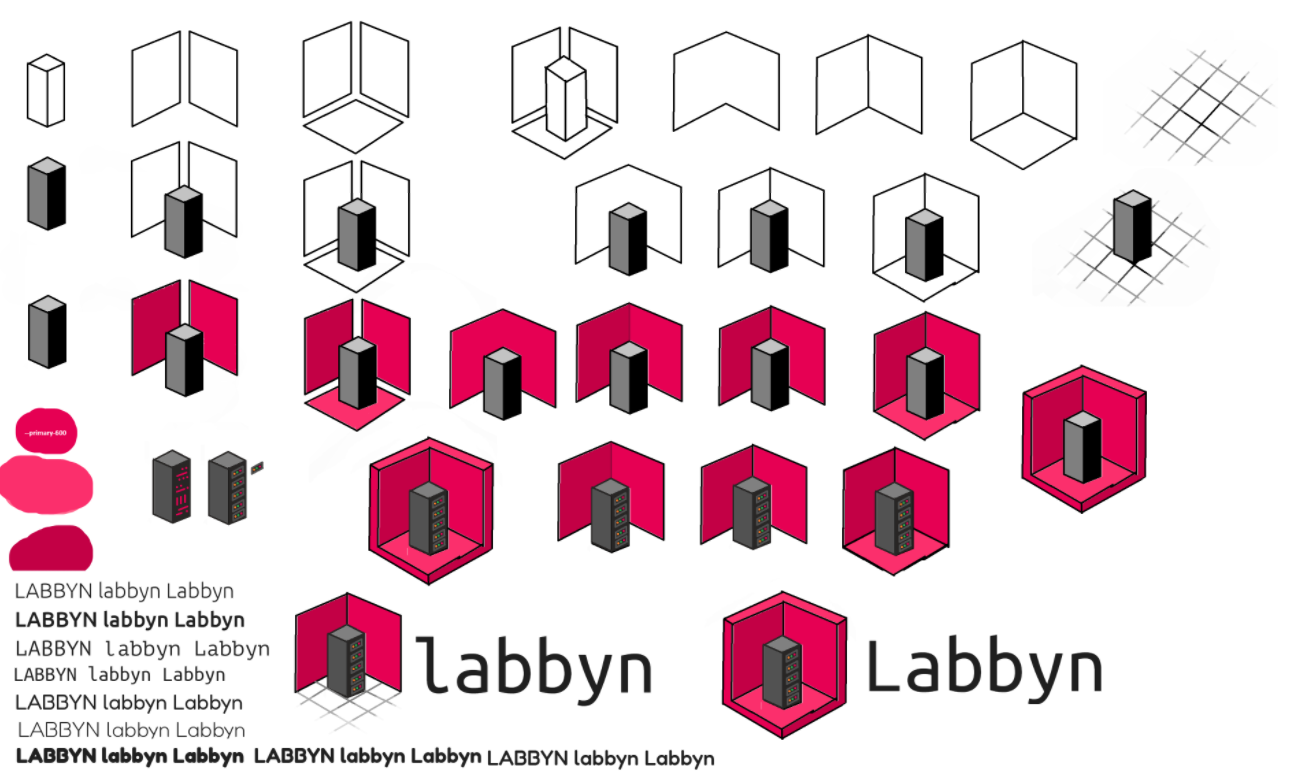
\includegraphics[width=\textwidth]{images/frontend/prototypowanie_loga_systemu.png}
    \caption{Proces prototypowania loga aplikacji (opracowanie własne)}
    \label{img:prototypowanie_loga}
\end{figure}


\section{Główne elementy budujące UI}

\subsection{Sidebar}
Główne centrum nawigacyjne panelu umiejscowione na krawędzi ekranu.
Służy do przełączania głównych modułów biznesowych i organizuje aplikację w spójny szkielet układu.
Znajdują się w nim:
\begin{itemize}
    \item \textbf{Command Search:} Globalne narzędzie wywoływane skrótem klawiszowym, które oferuje zaawansowane wyszukiwanie zasobów oraz wywoływanie szybkich akcji kontekstowych. Poprawia ono ergonomię pracy, pozwalając na prostą i szybką nawigację.
    \begin{figure}[H]
        \centering
        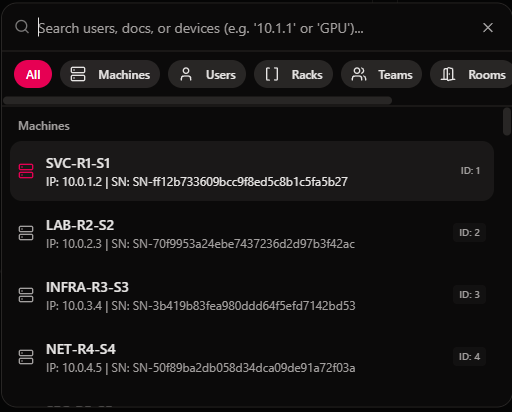
\includegraphics{images/frontend/search_bar.png}
        \caption{Mechanizm wyszukiwania obiektów w systemie (opracowanie własne)}
        \label{img:search_bar}
    \end{figure}
    \item \textbf{Zakładki:} Podstawowy element organizujący strukturę szczegółowych informacji. Na podstronach obiektów, zastosowanie zakładek minimalizuje konieczność przewijania długich stron i pozwala na ukrycie rzadziej wykorzystywanych paneli danych.
    \begin{figure}[H]
        \centering
        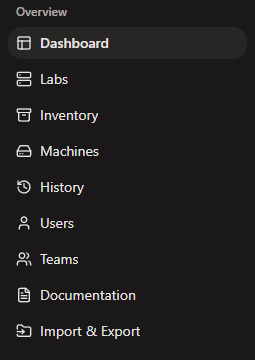
\includegraphics{images/frontend/sidebar_tabs.png}
        \caption{Zakładki dostępne z poziomu paska bocznego (opracowanie własne)}
        \label{img:sidebar_tabs}
    \end{figure}
    \item \textbf{Quick actions:} Służy do szybkiego zarządzania zasobami i infrastrukturą. Pozwala na wykonanie najczęściej używanych w systemie akcji przy użyciu jednego panelu. Centralizacja tych czynności zwiększa intuicyjność systemu jednocześnie minimalizując czas potrzebny na znalezienie pożądanej funkcjonalności.
    \begin{figure}[H]
        \centering
        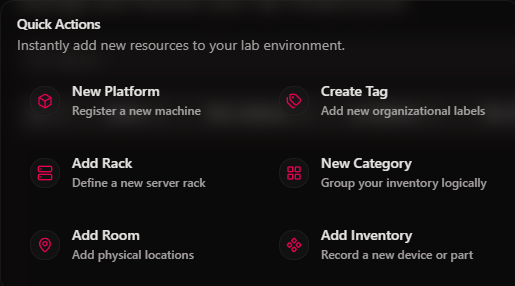
\includegraphics{images/frontend/quick_actions.png}
        \caption{Panel szybkich akcji (opracowanie własne)}
        \label{img:quick_actions}
    \end{figure}
    \item \textbf{Menu Użytkownika:} Stanowi element odpowiedzialny za prezentację informacji o aktualnie uwierzytelnionym użytkowniku, w szczególności jego nazwy. Kliknięcie tego elementu powoduje wyświetlenie menu kontekstowego pozwalającego na wylogowanie czy zmianę trybu wyświetlania aplikacji.
    \begin{figure}[H]
        \centering
        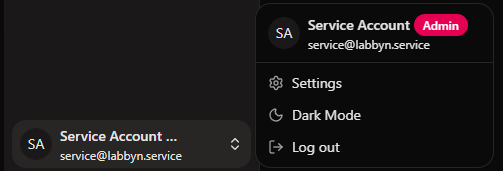
\includegraphics{images/frontend/user_menu.png}
        \caption{Menu użytkownika na pasku bocznym (opracowanie własne)}
        \label{img:user_menu}
    \end{figure}
\end{itemize}

\subsection{User Dashboard}
\par
Panel użytkownika pełni rolę podsumowania zasobów, do których aktualnie zalogowany użytkownik ma dostęp z tytułu przynależności do danych grup lub roli w systemie.
Dodatkowo panel zapewnia możliwość personalizacji widoku poprzez wykorzystanie mechanizmu “Customize View”, który umożliwia użytkownikowi dostosowanie prezentowanych informacji do jego indywidualnych potrzeb i preferencji.
\begin{figure}[H]
    \centering
    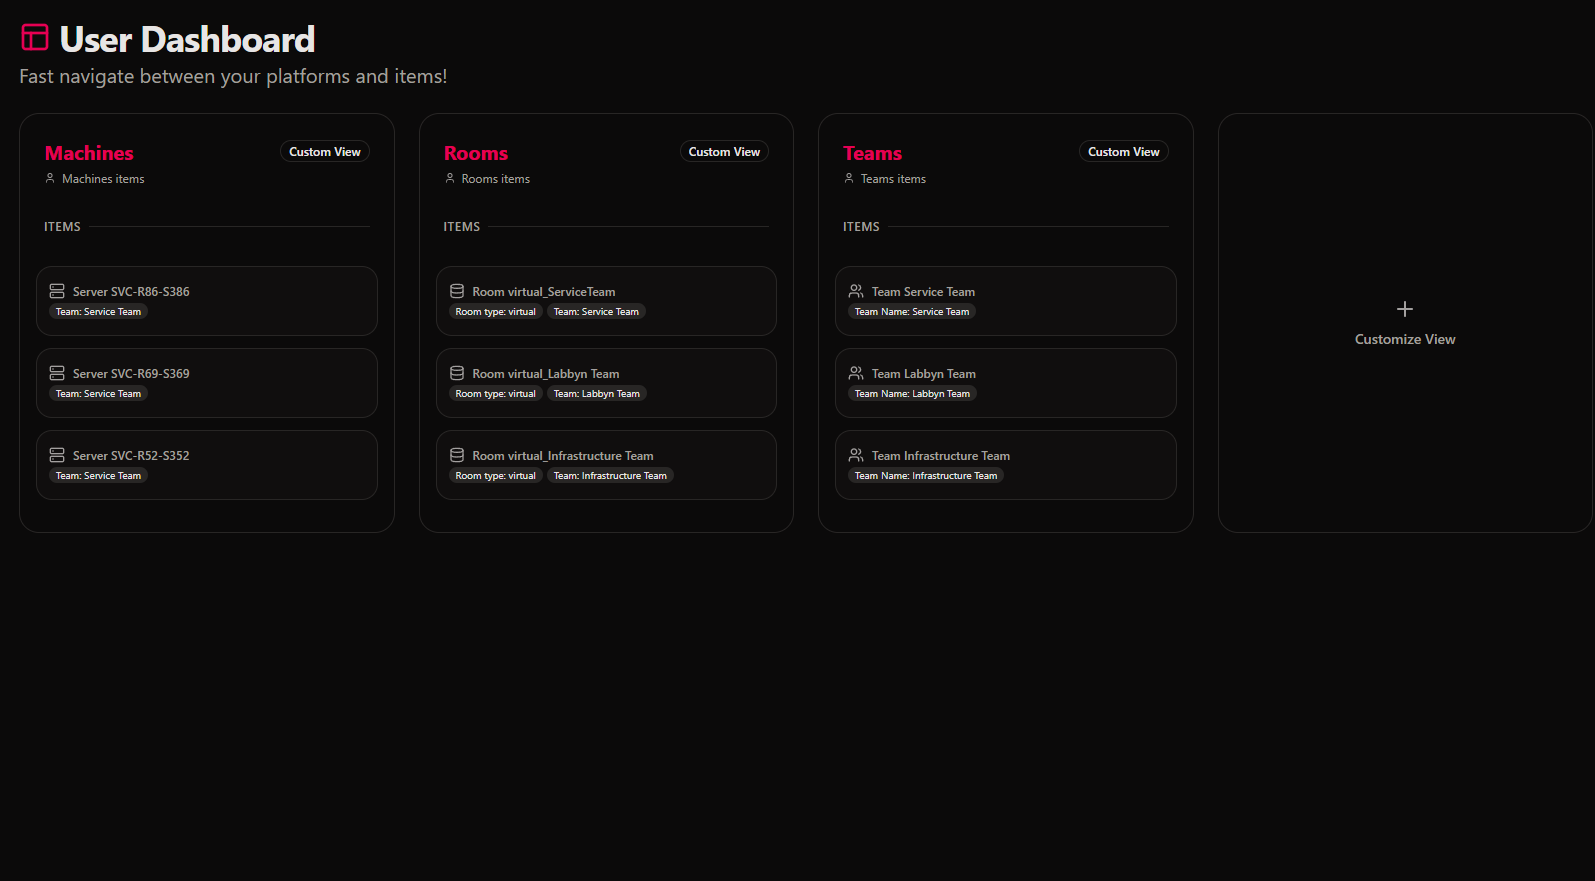
\includegraphics[width=\textwidth]{images/frontend/user_dashboard.png}
    \caption{Panel użytkownika (opracowanie własne)}
    \label{img:user_dashboard}
\end{figure}
\begin{figure}[H]
    \centering
    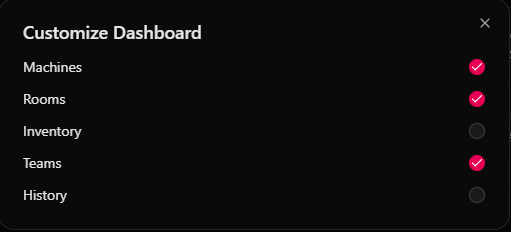
\includegraphics{images/frontend/user_dashboard_customize.png}
    \caption{Konfiguracja panelu użytkownika (opracowanie własne)}
    \label{img:user_dashboard_customize}
\end{figure}

\subsection{Labs}
\par
Panel laboratoriów zawiera informacje o dostępnych pomieszczeniach.
Każdy obiekt posiada krótkie podsumowanie w postaci: nazwy, właściciela oraz liczby szaf rackowych dostępnych w pomieszczeniu.
Posiada on także wyszukiwarkę pozwalającą na filtrowanie zwracanych wyników.
\begin{figure}[H]
    \centering
    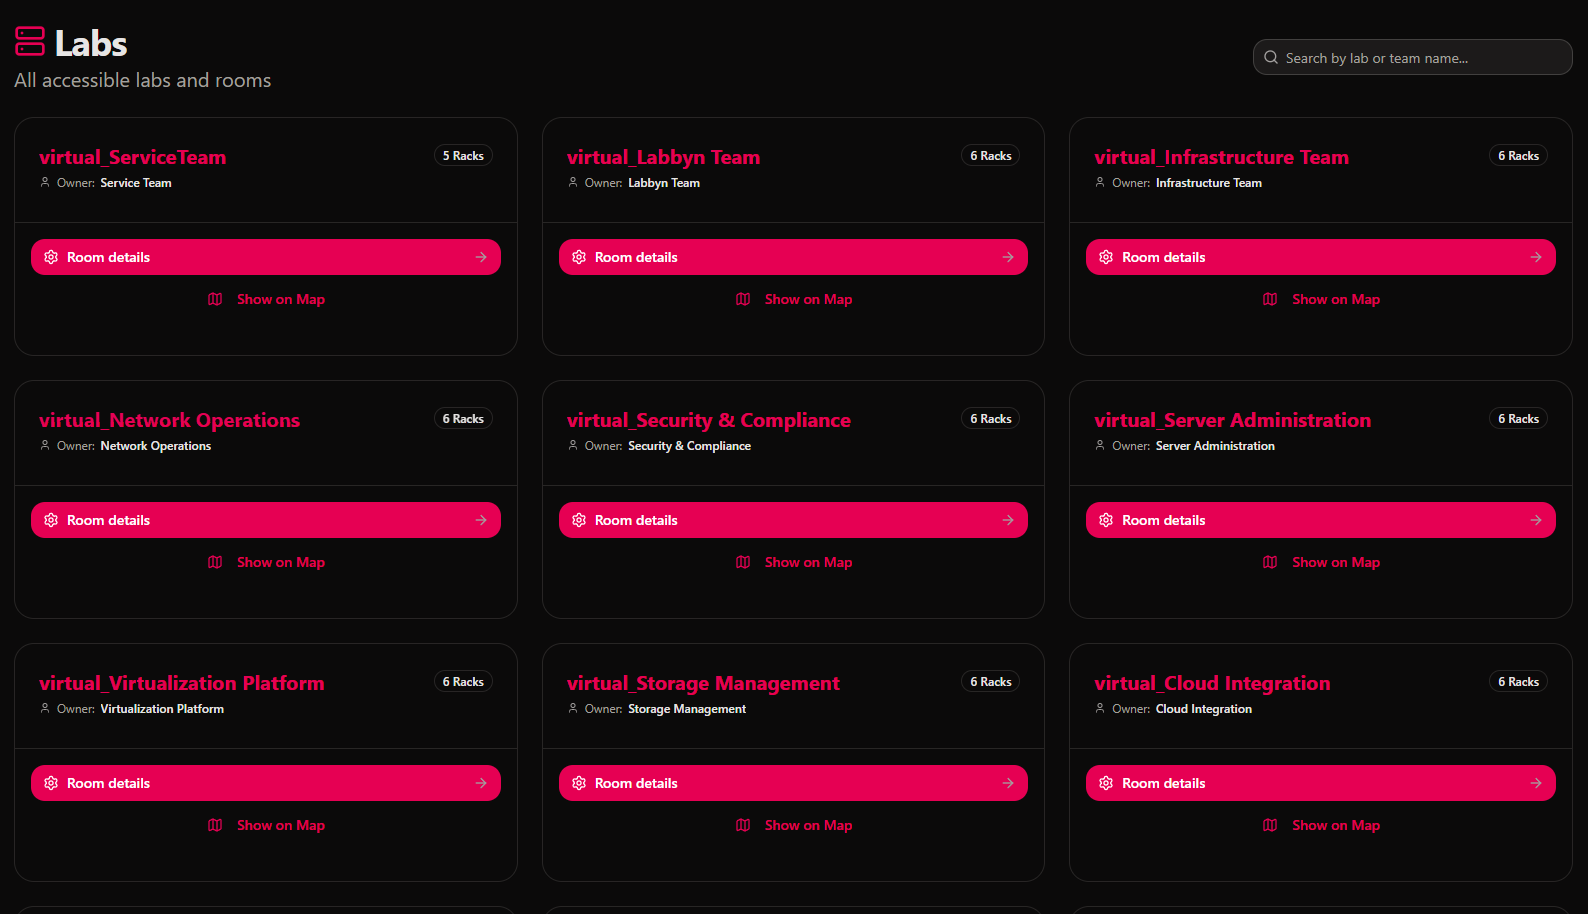
\includegraphics[width=\textwidth]{images/frontend/labs_overview.png}
    \caption{Panel "Labs" (opracowanie własne)}
    \label{img:labs_overview}
\end{figure}
\par
Niżej znajduje się przycisk szczegółów pomieszczenia, po kliknięciu w który użytkownik przenoszony jest na panel z listą szaf rackowych przypisanych do niego z możliwością wyszukiwania, filtrowania, sortowania oraz kontroli ilości zwracanych wyników.
\begin{figure}[H]
    \centering
    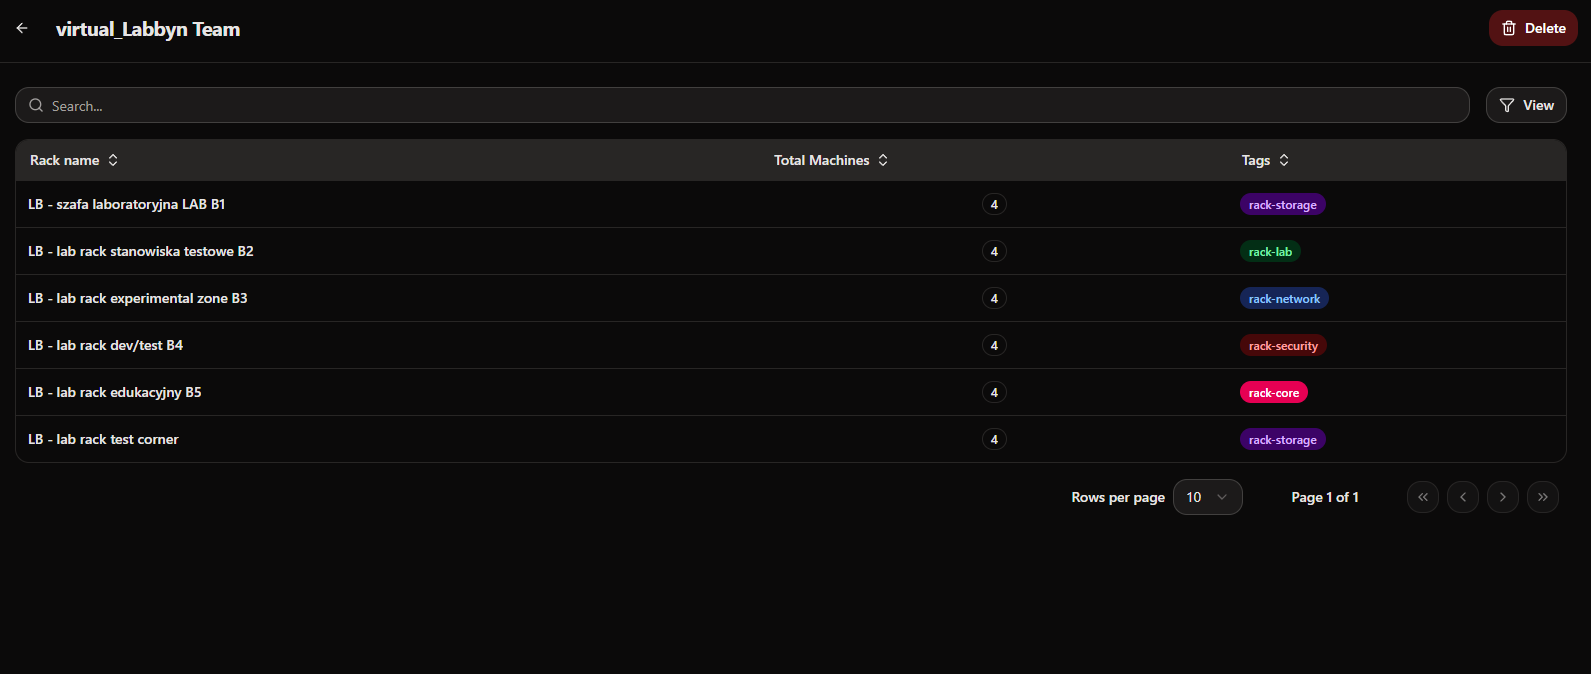
\includegraphics[width=\textwidth]{images/frontend/labs_details.png}
    \caption{Panel szczegółów pomieszczenia (opracowanie własne)}
    \label{img:labs_details}
\end{figure}
\par
Na dole obiektu widnieje przycisk “Show on Map”, który przekierowuje użytkownika do mapy przestrzennej wybranego pomieszczenia.

\subsection{Inventory}

\subsection{Machines}
\par
Moduł ten przeznaczony jest do zarządzania maszynami w systemie.
Głównym elementem jest tabela prezentująca szczegółowe informacje o urządzeniach.
Dla każdego obiektu wyświetlane są kluczowe atrybuty, takie jak: ID, nazwa, adres MAC, adres IP, przypisany zespół, numer seryjny czy notatka, których wyświetlanie można konfigurować przy pomocy przycisku “View”.
Tabela wspiera sortowanie otrzymanych wyników na podstawie kolumn z atrybutami.
W górnej części znajduje się pole wyszukiwania umożliwiające szybkie filtrowanie rekordów na podstawie wprowadzonych kryteriów.
\begin{figure}[H]
    \centering
    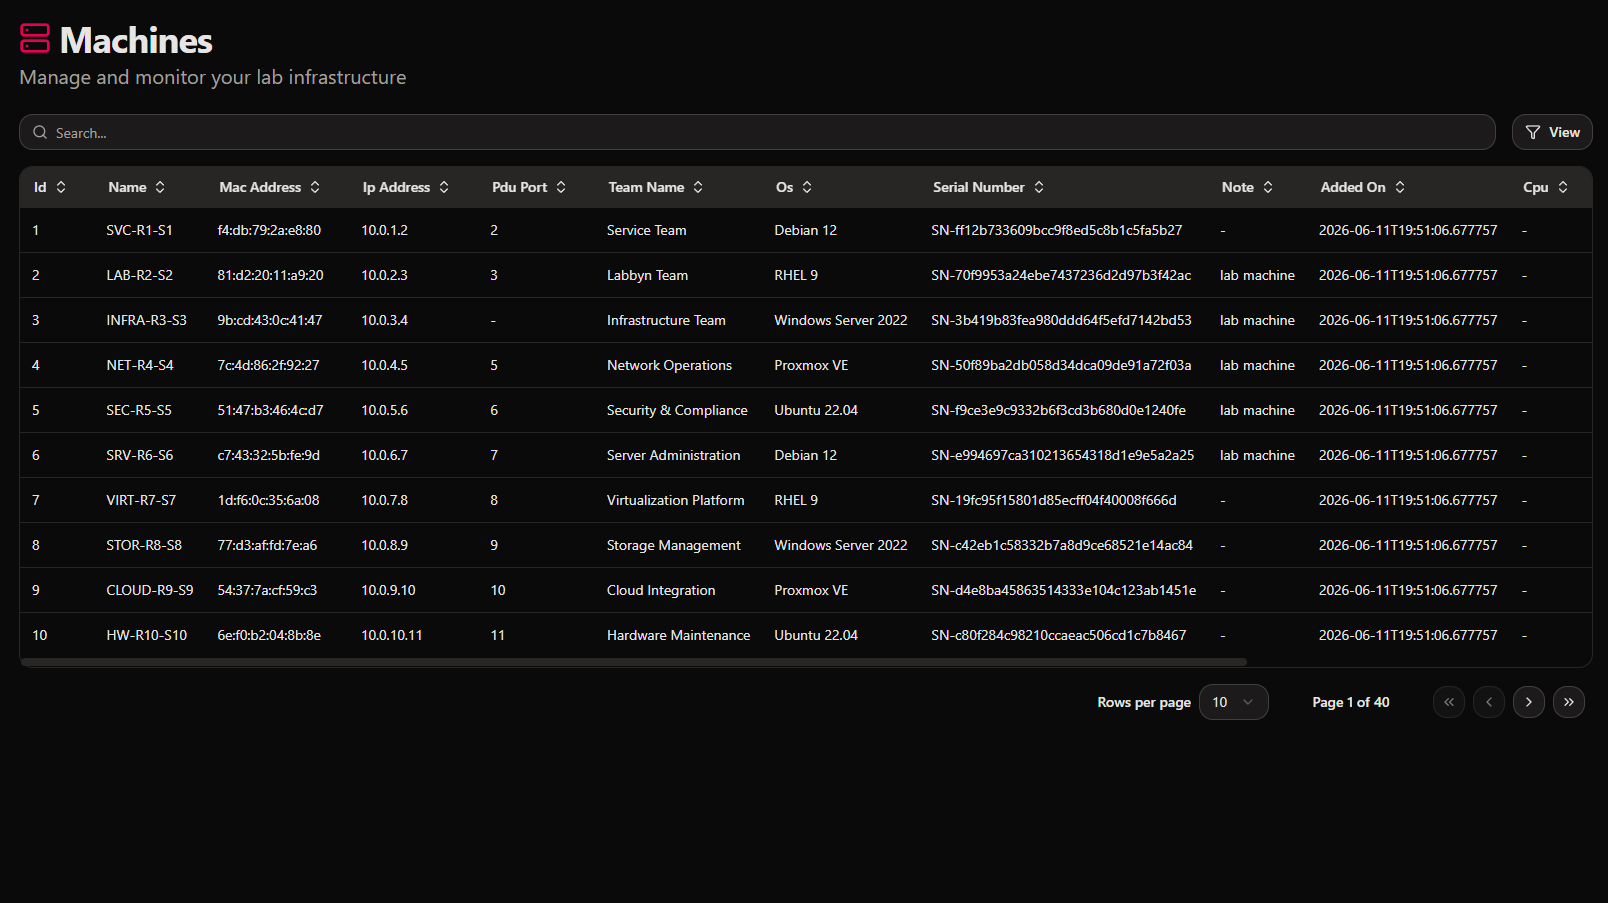
\includegraphics[width=\textwidth]{images/frontend/machines.png}
    \caption{Panel "Machines" (opracowanie własne)}
    \label{img:machines}
\end{figure}
\par
Każdy obiekt posiada odnośnik do strony ze szczegółami wybranego urządzenia.
Posiada on wszystkie informacje o maszynie dostępne w systemie: od szczegółów konfiguracji sprzętowej po lokalizację i dane telemetryczne pobierane z urządzenia w czasie rzeczywistym przy skonfigurowanym agencie Prometheus.
W górnej części znajdują się przyciski:
\begin{itemize}
    \item \textbf{Refresh host information} - służący do pobrania aktualnej konfiguracji sprzętowej urządzenia przy pomocy narzędzia Ansible
    \item \textbf{Manage monitoring agent} - pozwalające na instalację agenta Prometheus służącego do zbierania metryk
    \item \textbf{Edit} - zmieniające tryb przeglądania w tryb edycji informacji o sprzęcie
    \item \textbf{Delete} - pozwalający na usunięcie maszyny z systemu
\end{itemize}

\subsection{History}

\subsection{Users}

\subsection{Teams}

\subsection{Documentation}

\subsection{Import \& Export}




